\documentclass[11pt,a4paper]{ctexart}
\usepackage{ipara}
\usepackage{mathtools}
\usepackage{longtable}
\raggedbottom

\pagestyle{fancy}
\fancyhf{}
\lhead{\small 第三套数学自测卷}
\cfoot{\small 第 \thepage\ 页}
\renewcommand{\headrulewidth}{0.4pt}

\newcommand{\R}{\mathbb{R}}
\newcommand{\choiceworkspace}[1][3cm]{\vspace*{#1}}

\begin{document}

\begin{center}
  {\zihao{2}\bfseries 第三套数学自测卷}\\[2mm]
  \rule{0.86\linewidth}{0.5pt}
\end{center}

\setcounter{question}{0}

\section{单选题（本大题共 8 小题，每小题 5 分，共 40 分。在每小题给出的四个选项中，只有一项是符合题目要求的。）}

\autoquestion{若 $z=-3+4i$，则 $|z|=$ (\quad)}
\mcoptions[4]{12}{1}{$\sqrt5$}{5}
\choiceworkspace[2cm]

\autoquestion{若 $m\in \mathbb{R}$，$\lg 2^{51}=m+30.351$，$\lg 2\approx0.301$，则 $m=$ (\quad)}
\mcoptions[4]{$-16$}{$-15$}{$-14$}{$-13$}
\choiceworkspace[2cm]

\autoquestion{若命题 $p:x>2$，命题 $q:x<3$，则 $p$ 是 $\neg q$ 的 (\quad)}
\mcoptions[2]{充分不必要条件}{必要不充分条件}{充要条件}{既不充分也不必要条件}
\choiceworkspace[2.5cm]

\autoquestion{函数 $f(x)=3\tan\left(2x+\frac{\pi}{6}\right)$ 图像的对称中心坐标为 (\quad)}
\mcoptions[2]{$\left(\frac{k\pi}{2}-\frac{\pi}{12},0\right)(k\in\mathbb{Z})$}{$\left(\frac{k\pi}{2}-\frac{\pi}{3},0\right)(k\in\mathbb{Z})$}{$\left(\frac{k\pi}{4}-\frac{\pi}{12},0\right)(k\in\mathbb{Z})$}{$\left(\frac{k\pi}{4}-\frac{\pi}{6},0\right)(k\in\mathbb{Z})$}
\choiceworkspace[3cm]

\newpage

\autoquestion{如图，在棱长均为 2 的正四面体 $A-BCD$ 中，$E,F$ 分别为 $CD,BC$ 的中点，则 $AE,EF$ 所成角的余弦值为 (\quad)}
\sidefigureproblem{0.65}{}{%
  \begin{tikzpicture}[scale=1.2, >=stealth]
    \coordinate (B) at (0,0);
    \coordinate (C) at (2.2,0);
    \coordinate (D) at (0.9,0.6);
    \coordinate (A) at (1.1,1.9);
    
    \coordinate (E) at ($(C)!0.5!(D)$);
    \coordinate (F) at ($(B)!0.5!(C)$);
    
    \draw[dashed, gray] (B) -- (D);
    \draw[dashed, gray] (A) -- (D);
    \draw[dashed, gray] (C) -- (D);
    
    \draw[thick] (A) -- (B) -- (C) -- cycle;
    \draw[thick] (A) -- (C);
    
    \draw[thick, blue] (A) -- (E);
    \draw[thick, blue] (E) -- (F);
    \draw[dashed, blue] (A) -- (F);
    
    \fill (A) circle (1.2pt) node[above] {$A$};
    \fill (B) circle (1.2pt) node[below left] {$B$};
    \fill (C) circle (1.2pt) node[below right] {$C$};
    \fill (D) circle (1.2pt) node[right] {$D$};
    \fill (E) circle (1.2pt) node[right] {$E$};
    \fill (F) circle (1.2pt) node[below] {$F$};
  \end{tikzpicture}
}
\mcoptions[4]{$\frac{\sqrt3}{6}$}{$\frac{\sqrt{33}}6$}{$\frac13$}{$-\frac{\sqrt2}{6}$}
\choiceworkspace[3.5cm]

\autoquestion{若函数 $f(x)$ 的图象如下图所示，则 $f(x)$ 的解析式可能为 (\quad)}
\sidefigureproblem{0.65}{}{%
  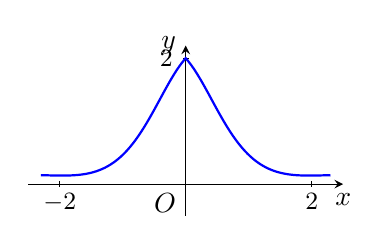
\begin{tikzpicture}[scale=0.8, >=stealth]
    \draw[->] (-2.5,0) -- (2.5,0) node[below] {$x$};
    \draw[->] (0,-0.5) -- (0,2.2) node[left] {$y$};
    \node[below left] at (0,0) {$O$};
    \foreach \x in {-2,2}
      \draw (\x,0.05) -- (\x,-0.05);
    \node[below] at (2,0) {\small $2$};
    \node[below] at (-2,0) {\small $-2$};
    \draw (0.05,2) -- (-0.05,2) node[left] {\small $2$};
    \draw[thick, blue, domain=-2.3:2.3, samples=151] 
      plot (\x, {exp(-1.14473*abs(\x)) + (cos(deg(\x))*cos(deg(\x)))/(\x*\x + 1)});
  \end{tikzpicture}
}
\mcoptions[2]{$f(x)=\pi^{|x|}+\frac{\sin x}{x^2+1}+1$}{$f(x)=\pi^{-|x|}+\frac{\cos^2x}{x^2+1}$}{$f(x)=\pi^{-|x|}+\frac{\sin x}{x^2+1}+1$}{$f(x)=\pi^{-|x|}+\frac{\cos x}{x^2+1}$}
\choiceworkspace[3.5cm]

\newpage

\autoquestion{已知某大厂的甲、乙车间生产的圆钢数之比为 $2:3$，现在要对甲、乙两个车间生产这种圆钢的直径进行误差抽检，具体要求为按比例分层抽检 50 根，若抽检的甲、乙车间圆钢的直径误差的平均值分别为 $1.1\text{ mm}, 1.05\text{ mm}$，误差的方差分别为 $0.5\text{ mm}^2, 0.45\text{ mm}^2$，则可以估计甲、乙车间的总体误差的方差约为 (\quad)}
\mcoptions[4]{$0.686\text{ mm}^2$}{$1.07\text{ mm}^2$}{$0.4706\text{ mm}^2$}{$0.475\text{ mm}^2$}
\choiceworkspace[4cm]

\autoquestion{如图，已知球 $O$ 的半径为 1，两个大圆面 $PAQ,PBQ$ 互相垂直，$\angle AOQ=\angle BOQ=\frac{2\pi}{3}$，若平面 $AOB$ 与平面 $PBQ$ 的夹角为 $\alpha$，则 (\quad)}
\sidefigureproblem{0.65}{}{%
  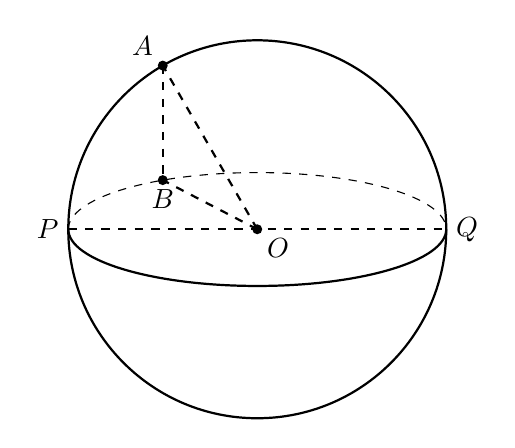
\begin{tikzpicture}[scale=1.2, >=stealth]
    % Outer sphere boundary
    \draw[thick] (0,0) circle (2);
    
    % Horizontal axis PQ
    \draw[dashed, thick] (-2,0) -- (2,0);
    \node[left] at (-2,0) {$P$};
    \node[right] at (2,0) {$Q$};
    \node[below right] at (0,0) {$O$};
    \fill (0,0) circle (1.5pt);
    
    % Horizontal ellipse (great circle)
    \draw[thick] (2,0) arc [start angle=0, end angle=-180, x radius=2, y radius=0.6];
    \draw[dashed] (-2,0) arc [start angle=180, end angle=0, x radius=2, y radius=0.6];
    
    % Coordinates
    \coordinate (A) at (-1, 1.732);
    \coordinate (B) at (-1, 0.52);
    
    % Connect OA, OB, AB
    \draw[dashed, thick] (0,0) -- (A);
    \draw[dashed, thick] (0,0) -- (B);
    \draw[dashed, thick] (A) -- (B);
    
    % Labels
    \fill (A) circle (1.5pt) node[above left] {$A$};
    \fill (B) circle (1.5pt) node[below] {$B$};
  \end{tikzpicture}
}
\mcoptions[2]{$AB=\frac{\sqrt6}{2},\tan\alpha=2$}{$AB=\frac{\sqrt6}{2},\tan\alpha=\frac{2\sqrt5}{5}$}{$AB=\frac{\sqrt3}{2},\tan\alpha=2$}{$AB=1,\tan\alpha=\frac12$}
\choiceworkspace[4cm]

\newpage

\section{多选题（本大题共 3 小题，每小题 6.5 分，共 18 分。在每小题给出的四个选项中，有多项符合题目要求。全部选对的得 6 分，部分选对的得部分分，有选错的得 0 分。）}

\autoquestion{在某次高三模拟考试后，数学老师统计了第一组的 8 名同学第 19 题的得分情况如下：$(7,9,5,8,5,3,3,3)$，第二组的 8 名同学第 19 题的得分情况如下：$(8,10,6,9,6,4,4,4)$，则 (\quad)}
\mcoptions[2]{第二组的平均数比较大}{两组的中位数之差的绝对值为 1}{两组的众数相等}{两组的极差相等}
\choiceworkspace[3.5cm]

\autoquestion{若将 4 张铁皮进行任意无重叠地切割，分别可以焊接成底面半径均为 1、高均为 2 的一个密闭圆锥和一个密闭圆柱、上下底面半径分别为 $(\frac12,\frac32)$、高为 2 的一个密闭圆台及直径为 2 的一个球，不考虑损耗，则体积与其表面积之比最大的是 (\quad)}
\mcoptions[4]{球}{圆锥}{圆柱}{圆台}
\choiceworkspace[4cm]

\autoquestion{在 $\triangle ABC$ 中，三个角 $A,B,C$ 所对的边分别为 $a,b,c$，其外接圆的半径为 $R$，若 $b^2=ac$，则 (\quad)}
\mcoptions[2]{$\triangle ABC$ 的面积为 $\frac{b^3}{4R}$}{$B\le \frac{\pi}{3}$}{$a+c<2b$}{$\frac{-1+\sqrt5}{2}<\frac ba<\frac{1+\sqrt5}{2}$}
\choiceworkspace[4.5cm]

\newpage

\section{填空题（本大题共 3 小题，每小题 5 分，共 15 分。）}

\autoquestion{从 $\{1,2,3,5\}$ 这四个数中随机取出 2 个不同的数，则它们差的绝对值为质数的概率为 \blank{1.5cm}。}
\choiceworkspace[4.5cm]

\autoquestion{若 $A=\{x \mid x=2k, k\in\mathbb{Z}\}$，$B=\{x \mid x=4k+1\text{ 或 }x=4k-1, k\in\mathbb{Z}\}$，则 $A\cap B = $ \blank{1.5cm}。}
\choiceworkspace[4.5cm]

\autoquestion{若方程 $e^{2x-1} = \frac{1-\ln x}{2x^2}$ 在 $(0,+\infty)$ 上有唯一解 $t$，则 $\frac{2t+\ln t}{2}$ 的值为 \blank{1.5cm}。}
\choiceworkspace[5cm]

\begin{freeblock}
  \section{解答题（本大题共 5 小题，共 77 分。解答应写出文字说明、证明过程或演算步骤。）}
  \stepcounter{question}\noindent\textbf{\arabic{question}.\ }已知 $\vec{a}=(1, \sin\theta), \vec{b}=(\cos\theta, t), \theta, t \in \mathbf{R}$.\\
  (1) 若 $t=-1, \vec{a}\perp\vec{b}$，求 $\theta$；\\
  (2) 若 $t=-\frac{\sqrt{3}}{4}, \vec{a}\parallel\vec{b}$，求 $\theta$.
  \answerblank[20cm]{解：}
\end{freeblock}

\begin{freeblock}
  \stepcounter{question}\noindent\textbf{\arabic{question}.\ }在直三棱柱 $ABC-A_1B_1C_1$ 中，已知 $D$ 为 $AC$ 的中点，$AB_1 \cap A_1B = O$.\\
  (1) 求证：$OD \parallel \text{平面 } BCC_1B_1$；\\
  (2) 若 $AB=BB_1=\sqrt{10}, BC=\sqrt{2}, AC=2\sqrt{3}$，证明：$A_1B \perp \text{平面 } AB_1C_1$.
  \begin{center}
    \begin{tikzpicture}[scale=1.2, >=stealth]
      \coordinate (A1) at (0,0);
      \coordinate (B1) at (4,0);
      \coordinate (C1) at (2.5,-1.5);
      
      \coordinate (A) at (0,3);
      \coordinate (B) at (4,3);
      \coordinate (C) at (2.5,1.5);
      
      \coordinate (D) at ($(A)!0.5!(C)$);
      \coordinate (O) at ($(A)!0.5!(B1)$); 
      
      % Dashed lines (back face and internal)
      \draw[dashed, thick] (A1) -- (B1);
      \draw[dashed, thick] (A) -- (B1);
      \draw[dashed, thick] (A1) -- (B);
      \draw[dashed, thick] (O) -- (D);
      \draw[dashed, thick] (A) -- (C1); % For plane AB1C1
      
      % Solid lines
      \draw[thick] (A) -- (B) -- (C) -- cycle;
      \draw[thick] (A1) -- (C1) -- (B1);
      \draw[thick] (A) -- (A1);
      \draw[thick] (B) -- (B1);
      \draw[thick] (C) -- (C1);
      
      \fill (A) circle (1pt) node[above left] {\(A\)};
      \fill (B) circle (1pt) node[above right] {\(B\)};
      \fill (C) circle (1pt) node[above right] {\(C\)};
      \fill (A1) circle (1pt) node[below left] {\(A_1\)};
      \fill (B1) circle (1pt) node[below right] {\(B_1\)};
      \fill (C1) circle (1pt) node[below] {\(C_1\)};
      \fill (D) circle (1pt) node[above right] {\(D\)};
      \fill (O) circle (1pt) node[right] {\(O\)};
    \end{tikzpicture}
  \end{center}
  \answerblank[15cm]{解：}
\end{freeblock}

\begin{freeblock}
  \stepcounter{question}\noindent\textbf{\arabic{question}.\ }已知 $\alpha - \frac{\beta}{2}, \frac{\alpha}{2} - \beta$ 均为第一象限的角，且 $\sin\left(\alpha - \frac{\beta}{2}\right) = \frac{3}{5}, \cos\left(\frac{\alpha}{2} - \beta\right) = \frac{7}{25}$，求：\\
  (1) $\sin\frac{3(\alpha - \beta)}{2}$ 的值；\\
  (2) $\cos(\alpha + \beta)$ 的值.
  \answerblank[22.5cm]{解：}
\end{freeblock}

\begin{freeblock}
  \stepcounter{question}\noindent\textbf{\arabic{question}.\ }如图，在平面四边形 $ABCD$ 中，已知 $AC, BD$ 交于 $O$, $AO = OC = \sqrt{2}, BD=2$, $\angle AOB = \frac{\pi}{4}$，且 $DO > BO$, 令 $\angle CDO = \alpha, \angle BAO = \beta$.\\
  (1) 判断：$AB=CD$ 是否成立？请说明理由；\\
  (2) 求 $\cos(\alpha - \beta)$ 的值；\\
  (3) 证明：当 $\beta = \frac{\pi}{6}$ 时，$D$ 位于 $\triangle ABC$ 外接圆的内部.
  \begin{center}
    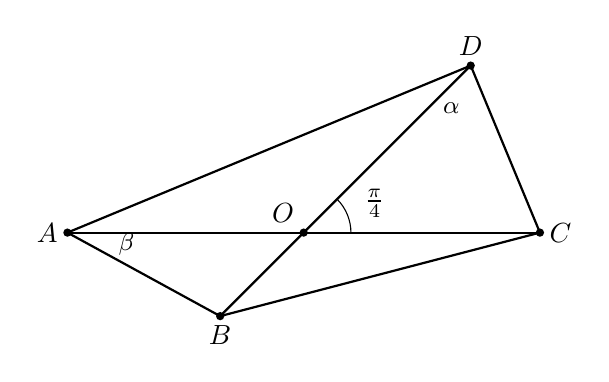
\begin{tikzpicture}[scale=1.5, >=stealth]
      \coordinate (O) at (0,0);
      \coordinate (A) at (-2, 0);
      \coordinate (C) at (2, 0);
      \coordinate (D) at (1.414, 1.414); 
      \coordinate (B) at (-0.707, -0.707); 
      
      \draw[thick] (A) -- (B) -- (C) -- (D) -- cycle;
      \draw[thick] (A) -- (C);
      \draw[thick] (B) -- (D);
      
      \fill (O) circle (1pt) node[above left] {$O$};
      \fill (A) circle (1pt) node[left] {$A$};
      \fill (B) circle (1pt) node[below] {$B$};
      \fill (C) circle (1pt) node[right] {$C$};
      \fill (D) circle (1pt) node[above] {$D$};
      
      \draw (0.4,0) arc (0:45:0.4);
      \node at (0.6, 0.25) {$\frac{\pi}{4}$};
      \node at (-1.5, -0.1) {\small $\beta$};
      \node at (1.25, 1.05) {\small $\alpha$};
    \end{tikzpicture}
  \end{center}
  \answerblank[17.5cm]{解：}
\end{freeblock}

\begin{freeblock}
  \stepcounter{question}\noindent\textbf{\arabic{question}.\ }在不透明的甲袋中装有相同的 6 个红色的乒乓球，其中 $a$ 个球上标有数字 1，$b$ 个球上标有数字 2，$6-a-b$ 个球上标有数字 3；在不透明的乙袋中装有相同的 3 个白色的乒乓球，其中 $m$ 个球上标有数字 1，$n$ 个球上标有数字 2，$3-m-n$ 个球上标有数字 3。\\
  (1) 若 $a=b=2, m=n=1$，分别从甲、乙袋中随机摸出一个球，求摸出两个球的数字相等的概率；\\
  (2) 若 $a=2, b=4, m=1, n=0$，从甲袋中有放回地随机摸出两个球，记下数字之和为 $p$，再从乙袋中有放回地随机摸出两个球，记下数字之和为 $q$，求 $p < q$ 的概率；\\
  (3) 若 $a=2, b=4, m=1, n=2$，将乙袋中的球倒入甲袋中，此时从甲袋中不放回地依次取 2 个小球，每次取 1 个，记事件 $M = \{$ 第一次取到的是红球 $\}$, 事件 $N = \{$ 第二次取到了标记数字 1 的球 $\}$, $M, N$ 是否相互独立？请说明理由。
  \answerblank[18cm]{解：}
\end{freeblock}

\end{document}
